\documentclass{article}
\usepackage{subcaption}
\usepackage{geometry}
\usepackage{ctex}
\usepackage{cite}
\usepackage{graphicx}
\usepackage{epstopdf}
\usepackage{amsmath,amsthm,amssymb,amsfonts}
\usepackage{booktabs}
\usepackage{pifont}
\usepackage{bm}

\begin{document} 
    \noindent \large \textbf{1.如图,在四边形ABCD中,AC与BD交于点O,AB=AC,AD=CD,\bm{$\angle $}ACB=2\bm{$\angle $}ACD,OA:OC=3:2,求\bm{$\frac{\text{OB}}{\text{OD}}$}的值}\\\\
    \begin{figure}[ht]
        \centering
        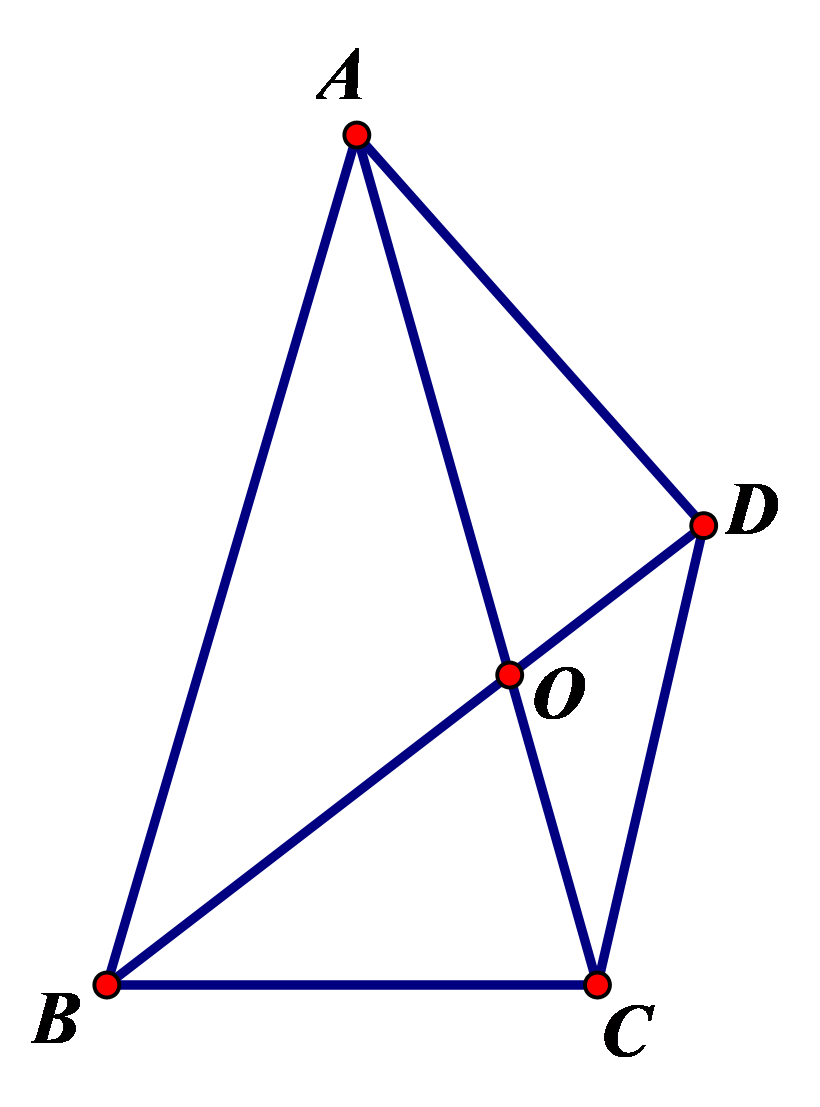
\includegraphics[scale=0.2]{1.png}
    \end{figure}\\
    解:设AB=5$x$,OA=3$x$,OC=2$x$,OD=$y$,OB=$ky$,BD=$(k+1)y$\\
    $\because $\quad $\angle $ADC=180$^{\circ }$-$\angle $ACD-$\angle $CAD=180$^{\circ}$-2$\angle $ACD,$\angle $ABC=$\angle $ACB=2$\angle $ACD \\
    $\therefore $\quad ABCD四点共圆 \\
    $\therefore $\quad $\angle $OCD=$\angle $CAD=$\angle $CBD \\
    $\therefore $\quad $\bigtriangleup $BDC$\sim $$\bigtriangleup $CDO \\
    $\therefore $\quad $\frac{\text{BD}}{\text{CD}}=\frac{\text{CD}}{\text{OD}}$,$\frac{\text{BC}}{\text{CO}}=\frac{\text{BD}}{\text{CD}}$\\
    $\therefore $\quad CD=$\sqrt{k+1}y$,BC=$2\sqrt{k+1}x$ \\
    又$\because $\quad 由托勒密定理:AB$\cdot $CD+AD$\cdot $BC=AC$\cdot $BD,且AB=AC,AD=CD \\
    $\therefore $\quad $5x\cdot\sqrt{k+1}y+2\sqrt{k+1}x\cdot\sqrt{k+1}y=5x\cdot (k+1)y$ \\
    $\therefore $\quad 解得:$k=\frac{16}{9}$ \\
    $\therefore $\quad $\frac{\text{OB}}{\text{OD}}=\frac{16}{9}$
    \newpage
    \noindent \textbf{2.如图,在等腰梯形ABCD中,AD//BC,AB=AD=CD,E是BC上一点,且\bm{$\angle $}ABE=\bm{$\angle $}AED,连接AC、BD交于点O,AC交DE于点G,BD交AE于点F,求证:\bm{$\frac{\text{AE}}{\text{AG}}=\frac{\text{DE}}{\text{DF}}$}} \\
    \begin{figure}[ht]
        \centering
        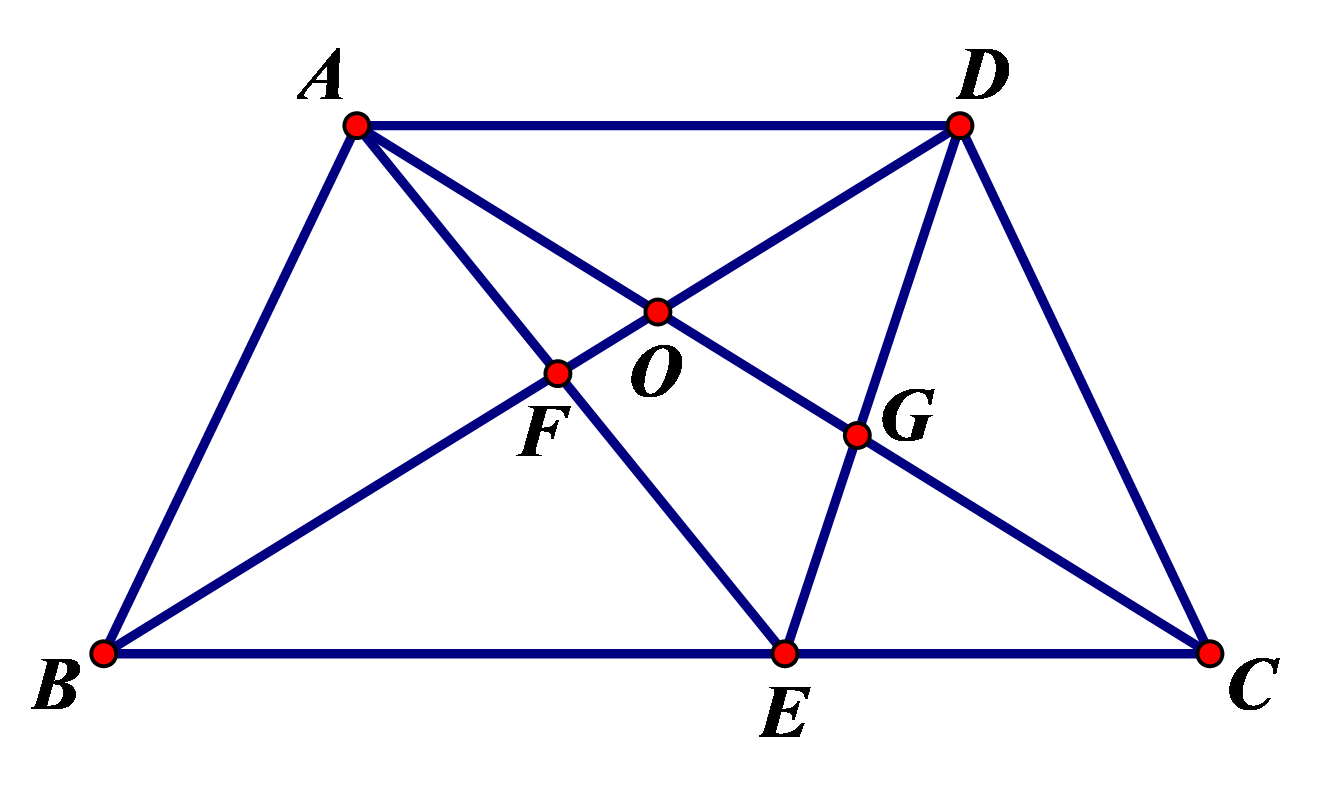
\includegraphics[scale=0.2]{2.png}
    \end{figure}\\
    证:在AE上取一点H,使得DF=DH \\
    \begin{minipage}[b]{0.65\linewidth}
        $\because $\quad AD//BC,AD=CD=AB \\
        $\therefore $\quad $\angle $BCA=$\angle $DBC=$\angle $ABD=$\angle $ACD=$\angle $ADB=$\angle $DAC \\
        $\therefore $\quad $\angle $DOG=$\angle $OAD+$\angle $ODA=$\angle $ABD+$\angle $DBC=$\angle $ABC=$\angle $AED \\
        $\therefore $\quad OFEG四点共圆 \\
        $\therefore $\quad $\angle $DFH+$\angle $AGE=180$^{\circ }$ \\
        又$\because $\quad DF=DH \\
        $\therefore $\quad $\angle $DFH=$\angle $DHF \\
        又$\because $\quad $\angle $DHF+$\angle $DHE=180$^{\circ }$ \\
        $\therefore $\quad $\angle $DHE=$\angle $AGE 
    \end{minipage}
    \hfill
    \begin{minipage}[b]{0.35\linewidth}
        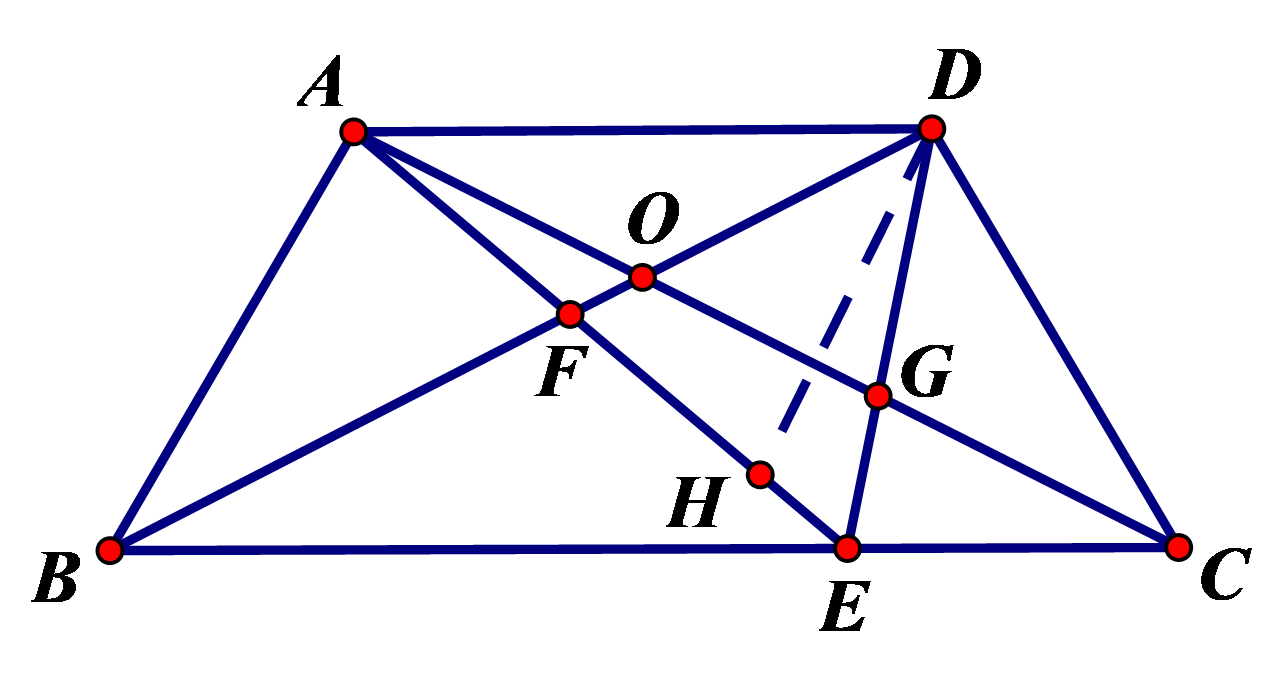
\includegraphics[scale=0.2]{2jie.png}
    \end{minipage}\\
    又$\because $\quad $\angle $DEH=$\angle $AEG \\
    $\therefore $\quad $\bigtriangleup \text{DEH}\sim \bigtriangleup \text{AEG}$ \\
    $\therefore $\quad $\frac{\text{AE}}{\text{AG}}=\frac{\text{DE}}{\text{DH}}$ \\
    $\therefore $\quad$\frac{\text{AE}}{\text{AG}}=\frac{\text{DE}}{\text{DF}}$ \\

    \newpage
    \noindent \textbf{3.如图,\bm{$\angle $}A=\bm{$\angle $}B=90\bm{$^{\circ }$},BC=2AD,用无刻度的直尺将ABCD补全成一个矩形} \\
    \begin{figure}[ht]
        \centering
        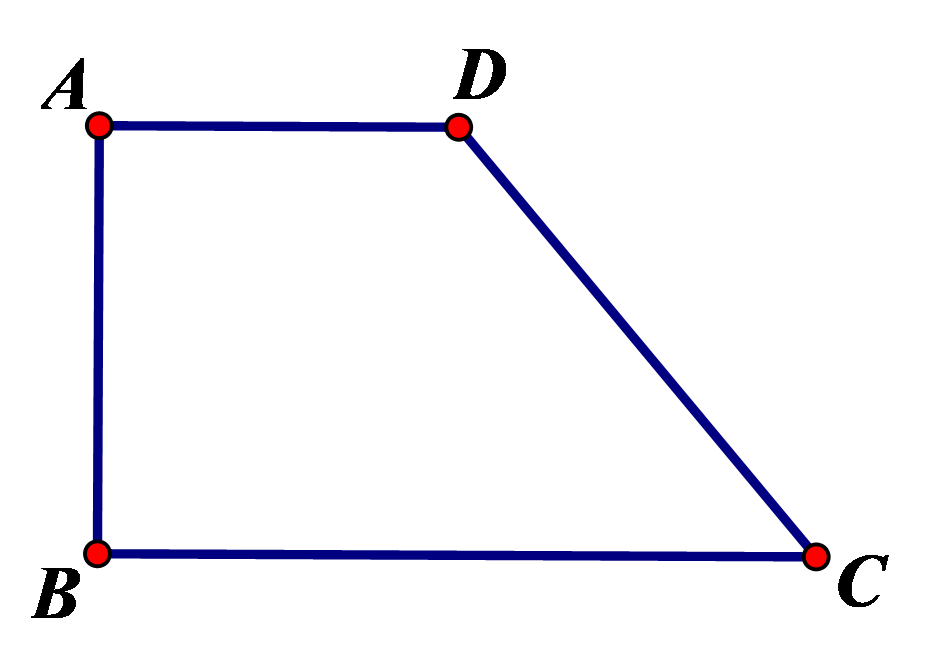
\includegraphics[scale=0.2]{3.png}
    \end{figure}\\
    \begin{figure}[ht]
        \centering
        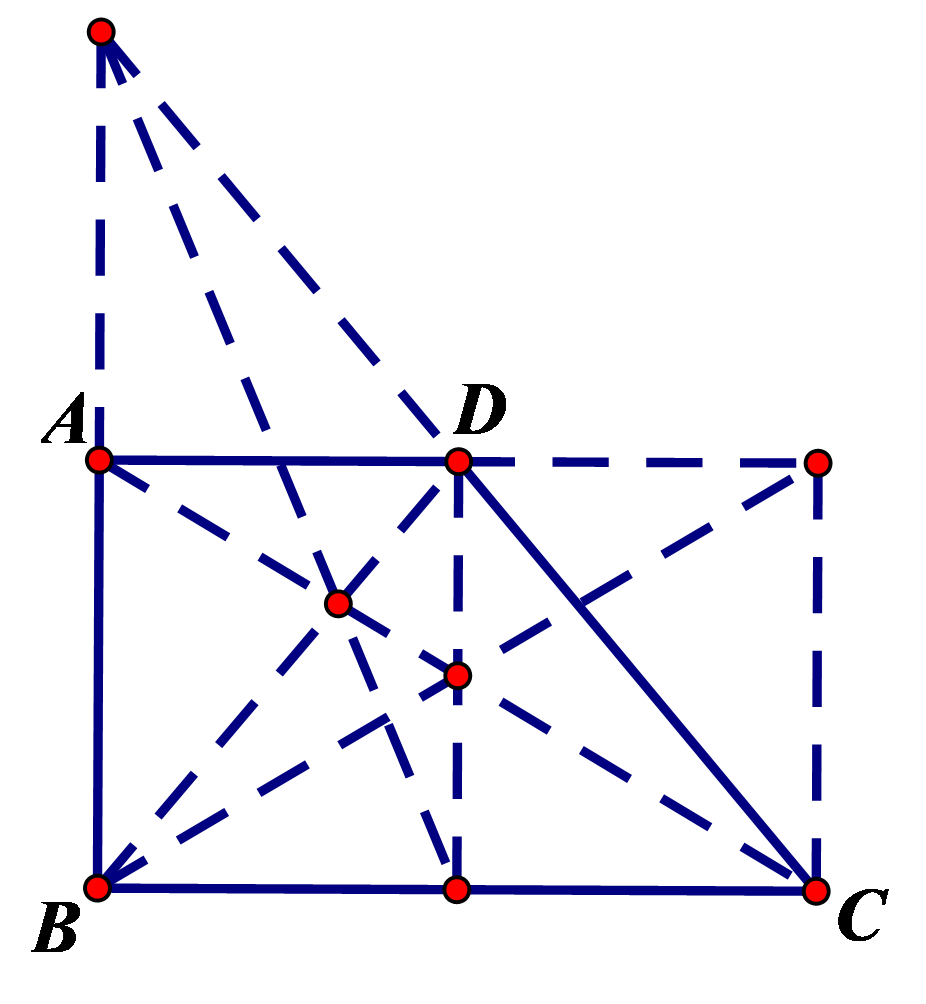
\includegraphics[scale=0.2]{3jie.png}
    \end{figure}\\

    \newpage
    \noindent \textbf{4.如图,在半圆中,O是圆心,AB是直径,E、F是\bm{${\stackrel{{\mbox{$\Large{\frown}$}}}{\text{AB}}}$}上的动点,连接OE、OF,\bm{$\angle $}EOF始终保持\bm{$\alpha $}不变
    ,作AG\bm{$\perp $}OE,垂足为G,延长AG交半圆于N,作BH\bm{$\perp $}OF,垂足为H,延长BH交半圆于M,BM与AN交于点K,连接MN(初中) \\
    (1)在E、F运动过程中,MN的长度是否为定值?若是,探求MN与AB的数量关系(用含\bm{$\alpha $}的三角函数表示);若不是,请说明理由 \\
    (2)若\bm{$\sin \alpha =\frac{\sqrt{7}}{3}$},OA=4,求\bm{$S_{\bigtriangleup \text{MKN}}$}的最大值} \\
    \begin{figure}[ht]
        \centering
        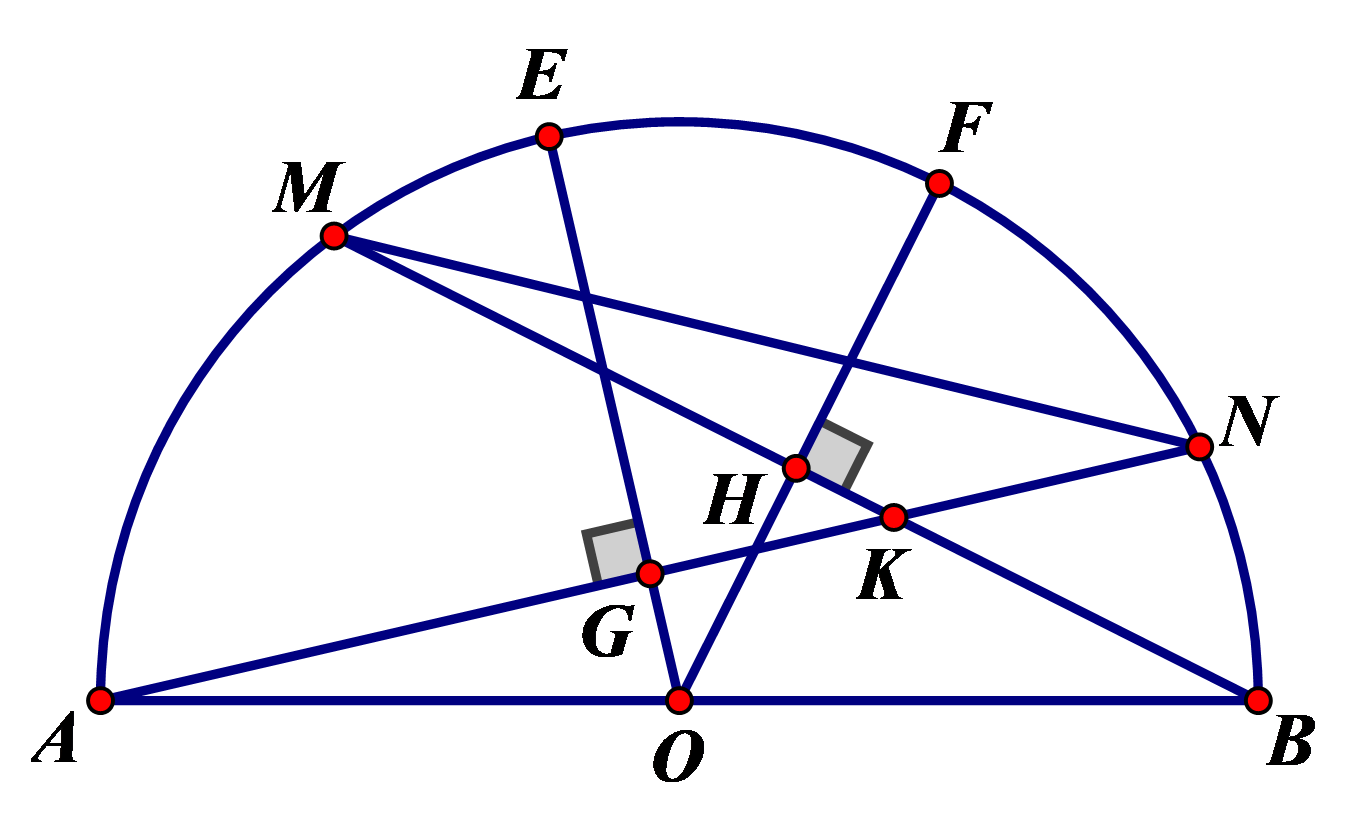
\includegraphics[scale=0.2]{4.png}
    \end{figure}\\
    解:(1)是定值\\
    $\because $\quad AN$\perp $OE,BM$\perp $OF \\
    $\therefore $\quad ${\stackrel{{\mbox{$\Large{\frown}$}}}{\text{BF}}}={\stackrel{{\mbox{$\Large{\frown}$}}}{\text{MF}}}$,${\stackrel{{\mbox{$\Large{\frown}$}}}{\text{AE}}}={\stackrel{{\mbox{$\Large{\frown}$}}}{\text{NE}}}$ \\
    \begin{minipage}[b]{0.65\linewidth}
        又$\because $\quad ${\stackrel{{\mbox{$\Large{\frown}$}}}{\text{AE}}}+{\stackrel{{\mbox{$\Large{\frown}$}}}{\text{BF}}}+{\stackrel{{\mbox{$\Large{\frown}$}}}{\text{EF}}}={\stackrel{{\mbox{$\Large{\frown}$}}}{\text{AB}}}$ \\
        $\therefore $\quad ${\stackrel{{\mbox{$\Large{\frown}$}}}{\text{MN}}}={\stackrel{{\mbox{$\Large{\frown}$}}}{\text{AN}}}+{\stackrel{{\mbox{$\Large{\frown}$}}}{\text{BM}}}
        -{\stackrel{{\mbox{$\Large{\frown}$}}}{\text{AB}}}=2\left({\stackrel{{\mbox{$\Large{\frown}$}}}{\text{AE}}}+{\stackrel{{\mbox{$\Large{\frown}$}}}{\text{BF}}}\right) -{\stackrel{{\mbox{$\Large{\frown}$}}}{\text{AB}}} \\
        \hspace*{0.5cm} =2\left({\stackrel{{\mbox{$\Large{\frown}$}}}{\text{AB}}}-{\stackrel{{\mbox{$\Large{\frown}$}}}{\text{EF}}}\right) -{\stackrel{{\mbox{$\Large{\frown}$}}}{\text{AB}}} \\
        \hspace*{0.5cm} ={\stackrel{{\mbox{$\Large{\frown}$}}}{\text{AB}}}-2{\stackrel{{\mbox{$\Large{\frown}$}}}{\text{EF}}}$\\
        $\therefore $\quad $\angle $MON=2$\left( 180^{\circ }-\alpha\right) -180^{\circ }$\\
        \hspace*{0.5cm} $=180^{\circ }-2\alpha $\\
        $\therefore $\quad $\angle $OMN=$\angle $ONM=$\alpha $ \\
        $\therefore $\quad MN=2$R\cos\alpha $=AB$\cos\alpha $
    \end{minipage}
    \hfill
    \begin{minipage}[b]{0.35\linewidth}
        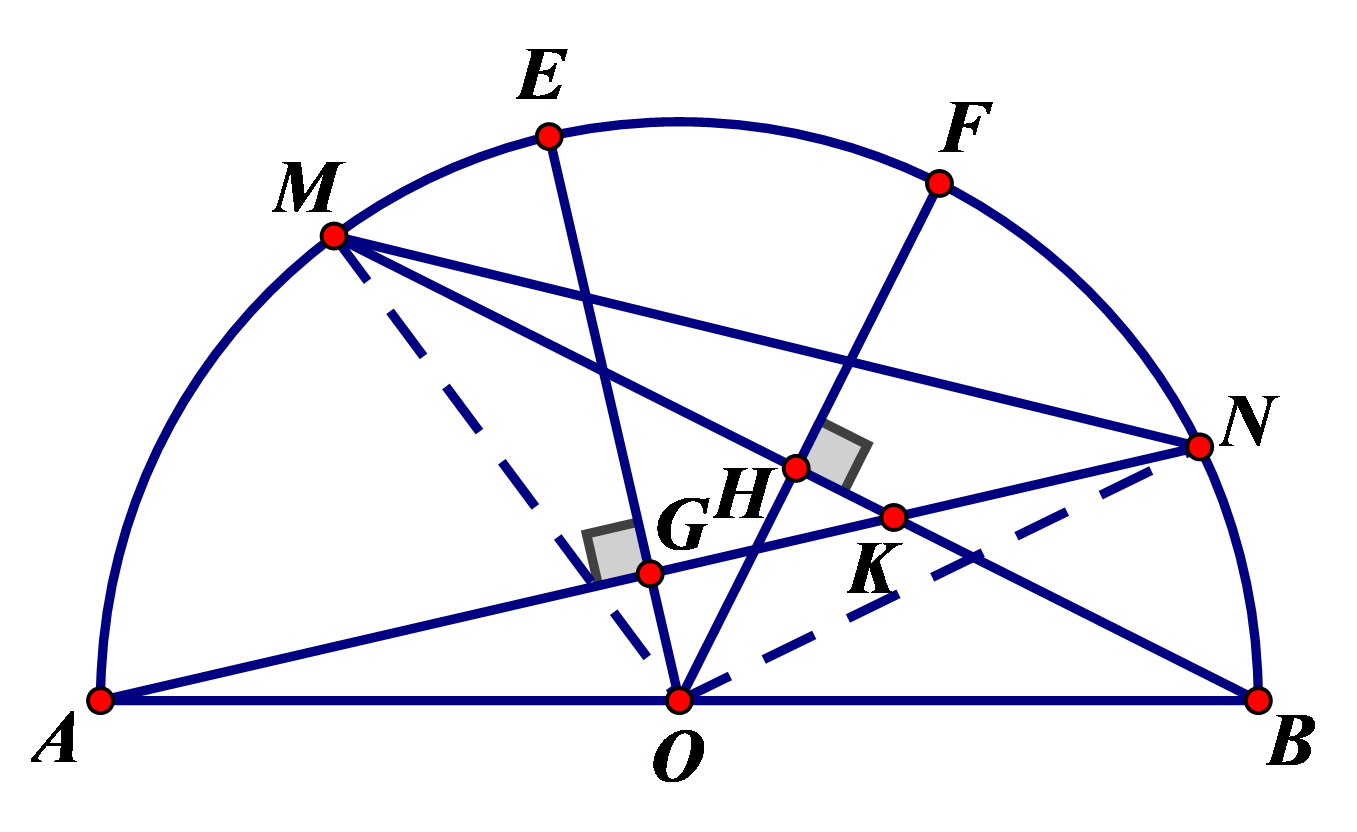
\includegraphics[scale=0.2]{4fuzhu.png}
    \end{minipage}
    \newpage
    \noindent (2)\quad $\because $\quad $\angle $KMN=$\angle $KAB,$\angle $KNM=$\angle $KBA \\
    $\therefore $\quad $\bigtriangleup $KMN$\sim $$\bigtriangleup $KAB \\
    $\therefore $\quad $\frac{S_{\bigtriangleup\text{KMN}}}{S_{\bigtriangleup\text{KAB}}}=\left(\frac{\text{MN}}{\text{AB}}\right) ^{2}=\left(\cos\alpha\right) ^{2}=1-\sin ^{2} \alpha = \frac{2}{9}$ \\
    又$\because $\quad 同(1)中推导可以得到:$\angle $AKB=$180^{\circ }-\alpha $ \\
    $\therefore $\quad $\angle $AKB为定值,K点在定弧上运动,当K到达弧顶时,即OK$\perp $AB时,$S_{\bigtriangleup\text{KAB}}$
    \hspace*{0.5cm} 最大 \\
    \begin{minipage}[htbp]{0.65\linewidth}
    $\because $\quad $\angle $AMK=$\angle $AOK=$90^{\circ }$ \\
    $\therefore $\quad AOKM四点共圆 \\
    $\therefore $\quad BK$\cdot $BM=BO$\cdot $BA=32 \\
    又$\because $\quad $\frac{\text{MK}}{\text{BK}}=\frac{\text{MN}}{\text{AB}}=\cos\alpha =\frac{\sqrt{2}}{3}$ \\
    $\therefore $\quad BK$\cdot $BM=BK$\left(\text{BK}+\text{MK}\right)$=$\left(1+\frac{\sqrt{2}}{3}\right)$BK$^{2}=32$ \\
    \hfill
    \end{minipage}
    \begin{minipage}[htbp]{0.35\linewidth}
        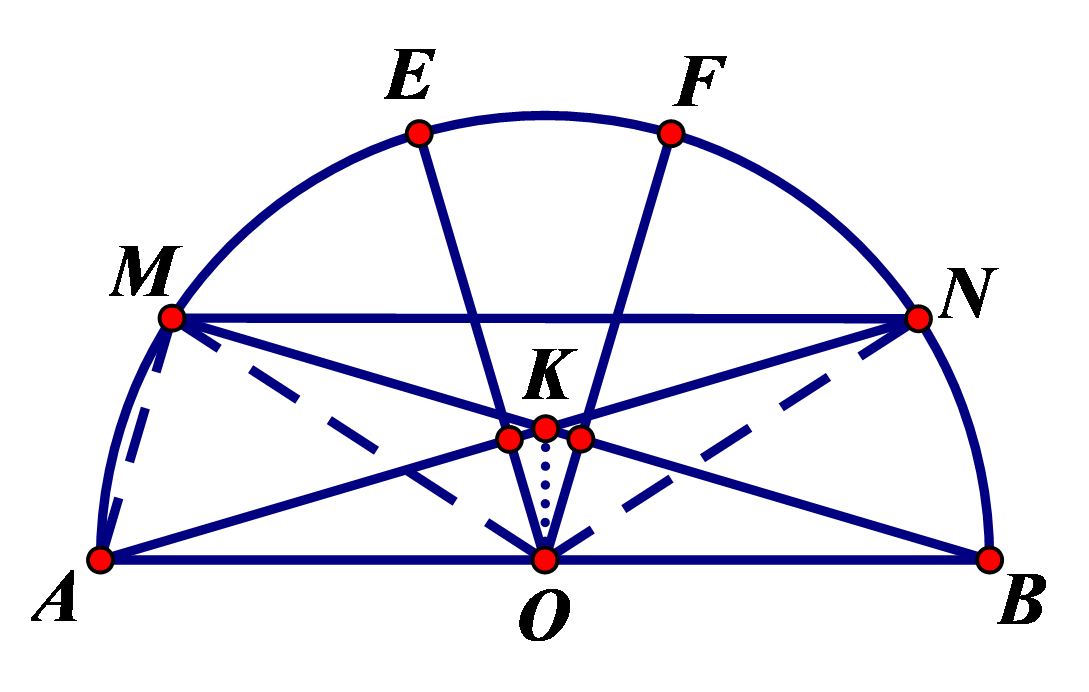
\includegraphics[scale=0.2]{4jie.png}
    \end{minipage}
    $\therefore $\quad BK$^{2}$=$\frac{32}{1+\frac{\sqrt{2}}{3}}$ \\
    又$\because $\quad $\angle $MKA=$180^{\circ }-\angle $AKB=$\alpha $ \\
    $\therefore $\quad MA=AK$\sin\alpha $=BK$\sin\alpha $=$\frac{\sqrt{7}}{3}$BK \\
    $\therefore $\quad $S_{\bigtriangleup\text{KAB}}=\frac{1}{2}\cdot \text{MA}\cdot \text{BK}=\frac{\sqrt{7}}{6}\text{BK}^{2}=\frac{48\sqrt{7}-16\sqrt{14}}{7}$ \\
    $\therefore $\quad $S_{\bigtriangleup\text{MKN}}=\frac{2}{9}S_{\bigtriangleup\text{KAB}}=\frac{96\sqrt{7}-32\sqrt{14}}{63}$,当OK$\perp $AB时取最大值 \\
    \textbf{(注:初中没学过二倍角公式)}
\end{document}